\documentclass[resume.tex]{subfiles}


\begin{document}
\section{Codage de canal}
\begin{center}
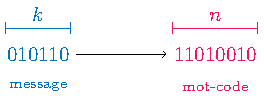
\includegraphics[scale=1,page=1]{drwg_1.pdf}
\end{center}
\begin{center}
\begin{tabular}{c|l}
$k$ & Nombre de bits à transmettre (information)\\\hline
$n$ & Nombre de bits transmis $n\geq k$
\end{tabular}
\end{center}
Information (bits à transmettre)
$$x=\begin{pmatrix}
x_{k-1} &
x_{k-2} &
\cdots &
x_1 &
x_0
\end{pmatrix}\in \mathbb{R}^{1\times k}$$

$$G_S=\begin{pmatrix}
\textcolor{RoyalBlue}{I_k} & \textcolor{OrangeRed}{P}
\end{pmatrix}=
\left(\begin{array}{cccc|cccc}
\textcolor{RoyalBlue}{1} & \textcolor{RoyalBlue}{0} & \cdots & \textcolor{RoyalBlue}{0} & \textcolor{OrangeRed}{x} & \cdots & \textcolor{OrangeRed}{x}\\
\textcolor{RoyalBlue}{0} & \textcolor{RoyalBlue}{1} & \cdots & \textcolor{RoyalBlue}{0} & \textcolor{OrangeRed}{x} & \cdots & \textcolor{OrangeRed}{x}\\
\vdots & \vdots & \ddots & \vdots & \vdots & \ddots & \vdots\\
\textcolor{RoyalBlue}{0} & \textcolor{RoyalBlue}{0} & \cdots & \textcolor{RoyalBlue}{1} & \textcolor{OrangeRed}{x} & \cdots & \textcolor{OrangeRed}{x}
\end{array}\right)\in\mathbb{R}^{k\times n}$$
$$H_s=\begin{pmatrix}
\textcolor{OrangeRed}{P^{T}} & \textcolor{RoyalBlue}{I_{n-k}}
\end{pmatrix}\in\mathbb{R}^{n-k\times n}$$
Encodage :
$$y=(xG_S)\bmod 2$$
Vérification (syndrome):
$$S=(yH_S^T)\bmod 2\quad \begin{cases}
=0 &\longrightarrow \text{ ok}\\
\neq 0 & \longrightarrow \text{ erreur}
\end{cases}$$
Décodage :
$$\hat{x}=y[0:k-1]$$


Propriétés
$$G_SH_S^T=0$$
\subsection{Codes linéaires}
La somme de deux codes valides donne un nouveau code valide
\subsection{Codes cycliques}
Un décalage vers la gauche ou vers la droite donne un autre code valide.\\
Un décalage d'un mot-code de longueur $n$ dans $\mathbb{R}_n[X]$ est similaire à une multiplication par $X$
\subsection{Générateur}
Un générateur permet, par des décalages cycliques et des sommes d'obtenir tous les mots-code.
\subsection{Générateur $\leftrightarrow$ matrice}
On peut créer la matrice en effectuant des décalages cycliques du générateur $g(x)$
$$\underset{k\times n}{\begin{pmatrix}
g_0 & g_1 & \cdots & g_{n-k} & 0 & 0\\
0 & g_0 & g_1 & \cdots & g_{n-k} & 0\\
0 & 0 & g_0 & g_1 & \cdots & g_{n-k}\\
\end{pmatrix}}$$
Avec le nombre de lignes correspondant à la longueur du message. Cette matrice n'est pas systématique. Il faut la manipuler si on veut obtenir la version systématique.
\end{document}